% Author: Izaak Neutelings (October 2019)
\documentclass[border=3pt,tikz]{standalone}
\usepackage{amsmath}
\usepackage{esvect} % \vv
\usepackage{tikz}
\usetikzlibrary{patterns,decorations.pathmorphing}
\tikzset{>=latex}
\usetikzlibrary{calc}
\usetikzlibrary{intersections}
\usetikzlibrary{arrows.meta}
\usetikzlibrary{angles,quotes} % for pic

\newcommand\Bc{{\mathrm{B}}}
\newcommand\Jpsi{{\mathrm{J}\!/\!\psi}}
\newcommand{\tikzAngleOfLine}{\tikz@AngleOfLine}
  \def\tikz@AngleOfLine(#1)(#2)#3{%
  \pgfmathanglebetweenpoints{%
    \pgfpointanchor{#1}{center}}{%
    \pgfpointanchor{#2}{center}}
  \pgfmathsetmacro{#3}{\pgfmathresult}%
}

%% ANGLE
%\tikzset{
%  pics/angarc/.style args={#1--#2--#3:#4}{
%    code = {
%      \tikzAngleOfLine(#2)(#1){\AngleStart}
%      \tikzAngleOfLine(#2)(#3){\AngleEnd}
%      \draw[red,<->] (#2)+(\AngleStart:#4) arc (\AngleStart:\AngleEnd:#4);
%    }
%  }
%}

\colorlet{beamcol}{orange!40!yellow!95!black}
\colorlet{SVcol}{green!50!blue!80!white}
\colorlet{Bccol}{green!80!blue!90!black}
\colorlet{Jpsicol}{red!90!black}
\colorlet{taucol}{orange!95!black}
\tikzset{
  ext/.style={shorten >=-#1,shorten <=-#1},
  ext/.default=1cm,
  smallarr/.style={{Latex[length={#1*4},width={#1*2.5}]}-{Latex[length={#1*4},width={#1*2.5}]}},
  smallarr/.default=1,
}



\begin{document}


%% Simple projection
%\begin{tikzpicture}
%  \coordinate (A) at (0,0);
%  \coordinate (B) at (4,3);
%  \coordinate (C) at (0.5,3);
%  \draw (A) -- (B);
%  \draw [blue] (C) -- ($(A)!(C)!(B)$);
%\end{tikzpicture}


% Bc -> J/psi tau nu
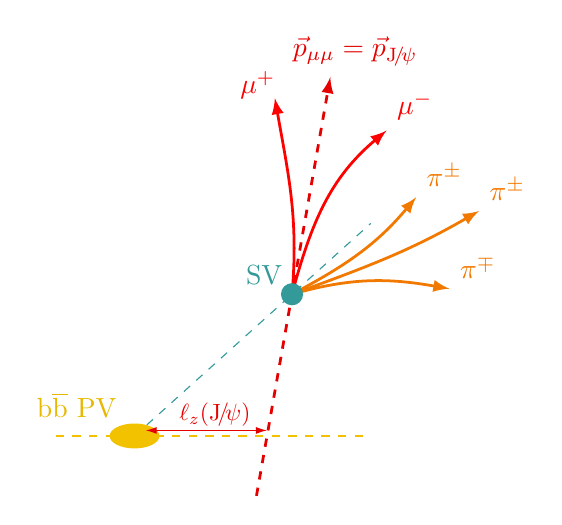
\begin{tikzpicture}
  
  \def\angJpsi{80}
  \coordinate (BL) at (-1,0);
  \coordinate (BR) at ( 3,0);
  \coordinate (PV) at ( 0,0);
  \coordinate (SV) at ( 2.0,1.8);
  \coordinate (Jp1) at ($(SV)+({\angJpsi-180}:2.6)$);
  \coordinate (Jp2) at ($(SV)+(\angJpsi:2.8)$);
  
  % DASHES
  \draw[beamcol,dashed,name path=beam]
    (BL) -- (BR);
  \draw[SVcol,dashed]
    (PV) -- (SV) -- ($(PV)!1.50!(SV)$);
  \draw[->,Jpsicol,dashed,line width=1,name path=mumu]
    (Jp1) -- (Jp2) node[right=9,above] {$\vec{p}_{\mu\mu} = \vec{p}_\Jpsi$};
  
  % MUONS
  \draw[->,red,line width=1]
    (SV) to[out=\angJpsi+5,in=-80] ++(\angJpsi+15:2.5) node[above left=-4] {$\mu^+$};
  \draw[->,red,line width=1]
    (SV) to[out=\angJpsi-5,in=-140] ++(\angJpsi-20:2.4) node[above right] {$\mu^-$};
  
  % PIONS
  \draw[->,taucol,line width=1]
    (SV) to[out=28,in=-130] ++(38:2.0) node[above right] {$\pi^\pm$};
  \draw[->,taucol,line width=1]
    (SV) to[out=20,in=-150] ++(24:2.6) node[above right] {$\pi^\pm$};
  \draw[->,taucol,line width=1]
    (SV) to[out=16,in=170] ++( 2:2.0) node[above right] {$\pi^\mp$};
  
  % BLOBS
  \fill[beamcol]
    (PV) ellipse (9pt and 4.5pt)
    node[beamcol!95!black,above left=3] {$\mathrm{b}\overline{\mathrm{b}}$ PV};
  \fill[SVcol]
    (SV) circle (4pt) node[above left] {SV};
  
  % LABELS
  \draw[smallarr,shorten <=4,Jpsicol,name intersections={of=beam and mumu,name=beam-mumu}]
    ([yshift=2]PV) -- ([yshift=2]beam-mumu-1) node[scale=0.85,right=6,midway,above=-2] {$\ell_z(\Jpsi)$};
  
  %\draw[smallarr,shorten <=4,Jpsicol] %,dashed
  %  (PV) -- ($(Jp1)!(PV)!(Jp2)$) node[scale=0.85,left=3,midway,below=1] {$\delta(\Jpsi)$};
  
\end{tikzpicture}


% Bs -> tau(mu) tau(3pi) 2nu
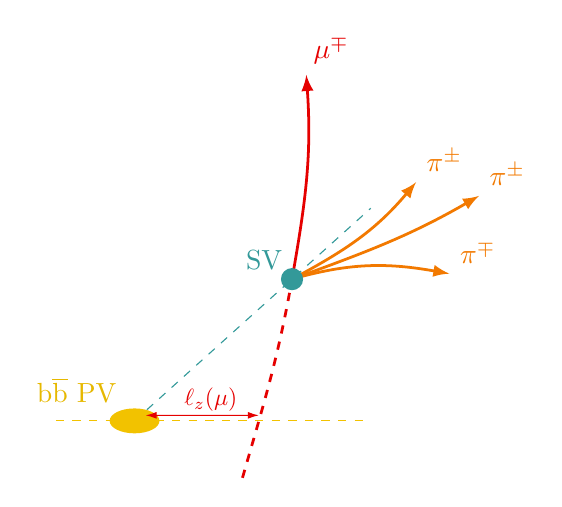
\begin{tikzpicture}
  
  \def\angJpsi{80}
  \coordinate (BL) at (-1,0);
  \coordinate (BR) at ( 3,0);
  \coordinate (PV) at ( 0,0);
  \coordinate (SV) at ( 2.0,1.8);
  \coordinate (Jp1) at ($(SV)+({\angJpsi-184}:2.6)$);
  \coordinate (Jp2) at ($(SV)+(\angJpsi+6:2.6)$);
  
  % DASHES
  \draw[beamcol,dashed,name path=beam]
    (BL) -- (BR);
  \draw[SVcol,dashed]
    (PV) -- (SV) -- ($(PV)!1.50!(SV)$);
    
  
  % MUONS
  \draw[Jpsicol,line width=1,dashed,name path=mumu]
    (Jp1) to[out=74,in=-100] (SV);
  \draw[->,Jpsicol,line width=1]
    (SV) to[out=80,in=-86] (Jp2) node[right=9,above] {$\mu^\mp$};
  
  % PIONS
  \draw[->,taucol,line width=1]
    (SV) to[out=28,in=-130] ++(38:2.0) node[above right] {$\pi^\pm$};
  \draw[->,taucol,line width=1]
    (SV) to[out=20,in=-150] ++(24:2.6) node[above right] {$\pi^\pm$};
  \draw[->,taucol,line width=1]
    (SV) to[out=16,in=170] ++( 2:2.0) node[above right] {$\pi^\mp$};
  
  % BLOBS
  \fill[beamcol]
    (PV) ellipse (9pt and 4.5pt)
    node[beamcol!95!black,above left=3] {$\mathrm{b}\overline{\mathrm{b}}$ PV};
  \fill[SVcol]
    (SV) circle (4pt) node[above left] {SV};
  
  % LABELS
  \draw[smallarr,shorten <=4,Jpsicol,name intersections={of=beam and mumu,name=beam-mumu}]
    ([yshift=2]PV) -- ([yshift=2]beam-mumu-1) node[scale=0.85,right=6,midway,above=-2] {$\ell_z(\mu)$};
  
  %\draw[smallarr,shorten <=4,Jpsicol] %,dashed
  %  (PV) -- ($(Jp1)!(PV)!(SV)$) node[scale=0.85,left=3,midway,below=1] {$\delta(\mu)$};
  
\end{tikzpicture}


% Bc -> J/psi tau nu
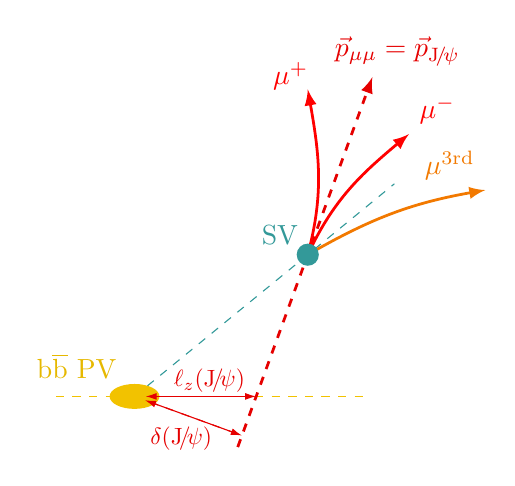
\begin{tikzpicture}
  
  \def\angJpsi{70}
  \coordinate (BL) at (-1,0);
  \coordinate (BR) at ( 3,0);
  \coordinate (PV) at ( 0,0);
  \coordinate (SV) at ( 2.2,1.8);
  \coordinate (Jp1) at ($(SV)+({\angJpsi-180}:2.6)$);
  \coordinate (Jp2) at ($(SV)+(\angJpsi:2.4)$);
  
  % DASHES
  \draw[beamcol,dashed,name path=beam]
    (BL) -- (BR);
  \draw[SVcol,dashed]
    (PV) -- (SV) -- ($(PV)!1.50!(SV)$);
  \draw[->,Jpsicol,dashed,line width=1,name path=mumu]
    (Jp1) -- (Jp2) node[right=9,above] {$\vec{p}_{\mu\mu} = \vec{p}_\Jpsi$};
  \draw[Jpsicol,dashed]
    (PV) -- ($(Jp1)!(PV)!(Jp2)$);
  
  % MUONS
  \draw[->,red,line width=1]
    (SV) to[out=\angJpsi+5,in=-80] ++(\angJpsi+20:2.1) node[above left=-4] {$\mu^+$};
  \draw[->,red,line width=1]
    (SV) to[out=\angJpsi-5,in=-140] ++(\angJpsi-20:2) node[above right] {$\mu^-$};
  \draw[->,taucol,line width=1]
    (SV) to[out=30,in=-170] ++(20:2.4) node[above left] {$\mu^\text{3rd}$};
  
  % BLOBS
  \fill[beamcol]
    (PV) ellipse (9pt and 4.5pt)
    node[beamcol!95!black,above left=3] {$\mathrm{b}\overline{\mathrm{b}}$ PV};
  \fill[SVcol]
    (SV) circle (4pt) node[above left] {SV};
  
  % LABELS
  \draw[smallarr,shorten <=4,Jpsicol,name intersections={of=beam and mumu,name=beam-mumu}]
    (PV) -- (beam-mumu-1) node[scale=0.85,right=6,midway,above=-2] {$\ell_z(\Jpsi)$};
  
  \draw[smallarr,shorten <=4,Jpsicol] %,dashed
    (PV) -- ($(Jp1)!(PV)!(Jp2)$) node[scale=0.85,left=3,midway,below=1] {$\delta(\Jpsi)$};
  
\end{tikzpicture}



% Bc -> J/psi tau nu
\begin{tikzpicture}
  
  \def\angJpsi{78}
  \def\angBc{48}
  \def\qlab{0.79}
  \coordinate (BL) at (-1,0);
  \coordinate (BR) at ( 4.5,0);
  \coordinate (PV) at ( 0,0);
  \coordinate (SV) at ( 3.4,1.6);
  \coordinate (Jp1) at ($(SV)+({\angJpsi-180}:3.2)$);
  \coordinate (Jp2) at ($(SV)+(\angJpsi:2.4)$);
  \coordinate (Bc1) at ($(SV)+({\angBc-180}:4.1)$);
  \coordinate (Bc2) at ($(SV)+(\angBc:3.3)$);
  \coordinate (SV2) at ($(PV)!1.50!(SV)$);
  
  % DASHES
  \draw[beamcol,dashed,name path=beam]
    (BL) -- (BR);
  \draw[SVcol,dashed]
    (PV) -- (SV) -- (SV2);
  \draw[->,Jpsicol,dashed,line width=1,name path=Jpsi]
    (Jp1) -- (Jp2) node[right=9,above] {$\vec{p}_{\mu\mu} = \vec{p}_\Jpsi$};
  \draw[->,Bccol,dashed,line width=1,name path=Bc]
    (Bc1) -- (Bc2) node[left=10,above right] {$\vec{p}_{\mu\mu\mu} = \vec{p}_\mathrm{B}$};
  
  % MUONS
  \draw[->,red,line width=1]
    (SV) to[out={\angJpsi+5},in={\angJpsi-150}] ++({\angJpsi+18}:2.1) node[above left=-4] {$\mu^+$};
  \draw[->,red,line width=1]
    (SV) to[out={\angJpsi-8},in={\angJpsi-210}] ++({\angJpsi-20}:2) node[right=2,above] {$\mu^-$};
  \draw[->,taucol,line width=1]
    (SV) to[out=38,in=-160] ++(29:3.1) node[above=2,above right] {$\mu^\text{3rd}$}; %{3^\text{rd}}
  
  % BLOBS
  \fill[beamcol]
    (PV) ellipse (9pt and 4.5pt)
    node[beamcol!95!black,above left=3] {$\mathrm{b}\overline{\mathrm{b}}$ PV};
  \fill[SVcol]
    (SV) circle (4pt) node[above left] {SV};
  
  % LABELS
  \draw[smallarr,shorten <=6,Bccol!90!black,
        name intersections={of=beam and Bc,name=beam-Bc}]
    ([yshift=2]PV) -- ([yshift=2]beam-Bc-1)
    node[scale=\qlab,right=14,midway,above=-1] {$\ell_z(\Bc)$};
  \draw[smallarr,shorten <=6,Jpsicol!90!black,
        name intersections={of=beam and Jpsi,name=beam-Jpsi}]
    ([yshift=-0.3]PV) -- ([yshift=-0.3]beam-Jpsi-1)
    node[scale=\qlab,left=15,above=-1] {$\ell_z(\Jpsi)$};
  \draw[smallarr,shorten <=4,Bccol] %,dashed
    (PV) -- ($(Bc1)!(PV)!(Bc2)$)
    node[scale=\qlab,left=3,midway,below=2] {$\delta(\Bc)$};
  \draw[smallarr,shorten <=6,Jpsicol] %,dashed
    (PV) -- ($(Jp1)!(PV)!(Jp2)$)
    node[scale=\qlab,below=4,left=10] {$\delta(\Jpsi)$};
  \draw[smallarr,shorten <=5,shorten >=2,SVcol!70!black] %,dashed
    ([shift={(120:0.01)}]PV) -- ([shift={(120:0.01)}]SV)
    node[scale=\qlab,midway,above=1] {$\ell$};
  
  % ANGLES
  \tikzAngleOfLine(SV)(Jp2){\angJp}
  \tikzAngleOfLine(SV)(Jp1){\angJpb}
  \tikzAngleOfLine(SV)(Bc2){\angBc}
  \tikzAngleOfLine(SV)(Bc1){\angBcb}
  \tikzAngleOfLine(SV)(SV2){\angSV}
  \draw[smallarr=0.9,blue] (SV)+(\angSV:0.8)
    node[scale=\qlab,right=2,below=0] {$\alpha(\Jpsi)$} arc (\angSV:\angJp:0.8);
  \draw[smallarr=0.9,blue] (SV)+(\angSV:1.4)
    node[scale=\qlab,right=7,below=-2] {$\alpha(\Bc)$} arc (\angSV:\angBc:1.4);
  \draw[smallarr=0.9,blue] (SV)+(\angJpb:0.9)
    node[scale=\qlab,right] {$\alpha(\Jpsi,\Bc)$} arc (\angJpb:\angBcb:0.9);
  
\end{tikzpicture}


% Bc -> J/psi tau nu
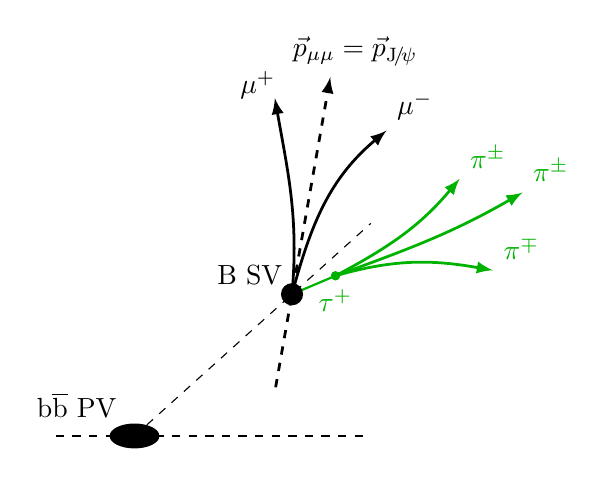
\begin{tikzpicture}
  
  \def\angJpsi{80}
  \coordinate (BL) at (-1,0);
  \coordinate (BR) at ( 3,0);
  \coordinate (PV) at ( 0,0);
  \coordinate (SV) at ( 2.0,1.8);
  \coordinate (Jp1) at ($(SV)+({\angJpsi-180}:1.2)$);
  \coordinate (Jp2) at ($(SV)+(\angJpsi:2.8)$);
  
  % DASHES
  \draw[dashed,name path=beam]
    (BL) -- (BR);
  \draw[dashed]
    (PV) -- (SV) -- ($(PV)!1.50!(SV)$);
  \draw[->,dashed,line width=1,name path=mumu]
    (Jp1) -- (Jp2) node[right=9,above] {$\vec{p}_{\mu\mu} = \vec{p}_\Jpsi$};
  
  % MUONS
  \draw[->,line width=1]
    (SV) to[out=\angJpsi+5,in=-80] ++(\angJpsi+15:2.5) node[above left=-4] {$\mu^+$};
  \draw[->,line width=1]
    (SV) to[out=\angJpsi-5,in=-140] ++(\angJpsi-20:2.4) node[above right] {$\mu^-$};
  
  % TAU
  \draw[thick,green!70!black]
    (SV) --++ (23:0.6) coordinate (T) node[midway,below right=-2] {$\tau^+$};
  \fill[green!70!black]
    (T) circle (0.06);
  
  % PIONS
  \draw[->,green!70!black,line width=1]
    (T) to[out=28,in=-130] ++(38:2.0) node[above right] {$\pi^\pm$};
  \draw[->,green!70!black,line width=1]
    (T) to[out=20,in=-150] ++(24:2.6) node[above right] {$\pi^\pm$};
  \draw[->,green!70!black,line width=1]
    (T) to[out=16,in=170] ++( 2:2.0) node[above right] {$\pi^\mp$};
  
  % BLOBS
  \fill[]
    (PV) ellipse (9pt and 4.5pt)
    node[above left=3] {$\mathrm{b}\overline{\mathrm{b}}$ PV};
  \fill[]
    (SV) circle (4pt) node[above left] {B SV};
  
  %\draw[smallarr,shorten <=4,Jpsicol] %,dashed
  %  (PV) -- ($(Jp1)!(PV)!(Jp2)$) node[scale=0.85,left=3,midway,below=1] {$\delta(\Jpsi)$};
  
\end{tikzpicture}


\end{document}